\documentclass[10pt,letterpaper]{article}

\usepackage{outlines}
\usepackage{amsmath}
\usepackage{tikz}
\usepackage{hyperref}
\usepackage{enumitem}
\usepackage{caption}
\usepackage{subcaption}
\DeclareCaptionOptionNoValue{centering}{\centering} % Make sure everything is centered in subs
\captionsetup[sub]{centering}

\usepackage{multirow}
\usepackage{cancel}
\usepackage{float}

\usepackage{parskip}

\usepackage{slantsc,lmodern}

\usepackage{pgfplotstable,booktabs}
\usepackage{textcomp}
\usepackage{gensymb}

\usepackage{paralist}

\usepackage{amsmath}
\usepackage{tikz}
\usepackage{hyperref}

\usepackage[paper=a4paper,margin=1in]{geometry}

\makeatletter
\g@addto@macro\@floatboxreset\centering
\makeatother

\newcommand{\volume}{{\ooalign{\hfil$V$\hfil\cr\kern0.08em--\hfil\cr}}}




\author{Thaddeus Hughes \\ hughes.thad@gmail.com \\ thaddeus-maximus.github.io}
\date{\today}
\title{Center-to-center calculation for power transmission belts}

\begin{document}
	\maketitle
	
	\begin{abstract}
		Belts are pretty easy to use and calculate the appropriate distances for. When this center distance is calculated and manufactured properly, they should not require adjustment.
	\end{abstract}
	
	
	\begin{figure}[H]
	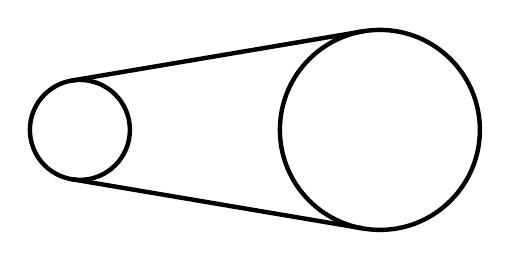
\begin{tikzpicture}[x=0.5in,y=0.5in]
		\draw[ultra thick] (0,0) circle (0.5);
		\draw[ultra thick] (3,0) circle (1);
		\draw[ultra thick] (-.08333, .4930) -- (2.83333, .9860);
		\draw[ultra thick] (-.08333, -.4930) -- (2.83333, -.9860);
	\end{tikzpicture}
	\caption{Belt and Sprockets}
	\end{figure}

	\begin{figure}[H]
	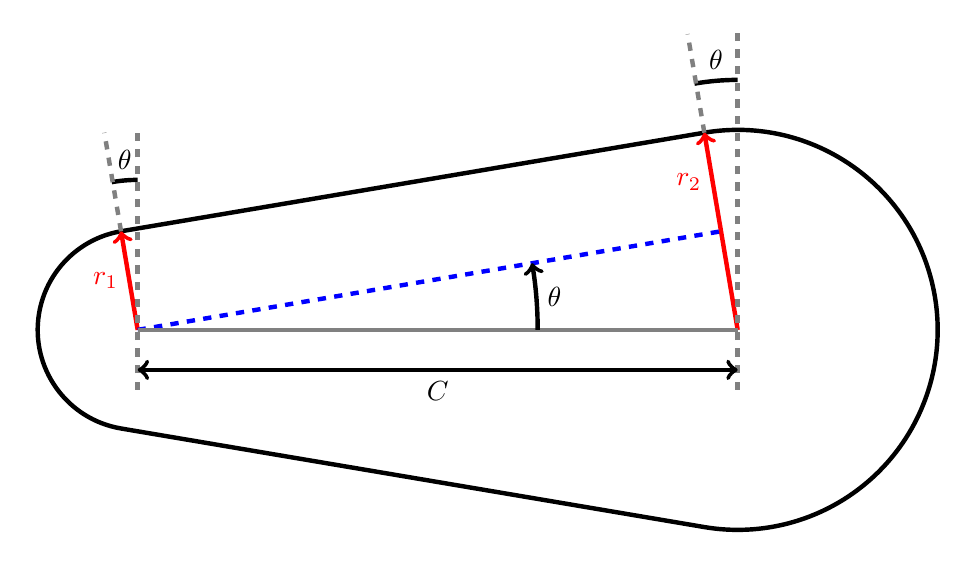
\begin{tikzpicture}[x=1.0in,y=1.0in]
		\draw[black, ultra thick] (-.08333, .4930) -- (2.83333, .9860) arc (99.594:-99.594:1) -- (-.08333, -.4930) arc (260.406:99.594:0.5) -- cycle;
		\draw[red, ultra thick, ->] (0,0) -- (-.08333, .4930) node[pos=0.5, left]{$r_1$};
		\draw[red, ultra thick, ->] (3,0) -- (2.83333, .9860) node[pos=0.75, left]{$r_2$};
		\draw[black, ultra thick] (0,0.75) arc (90:99.9594:0.75) node[pos=0.5, above]{$\theta$};
		\draw[black, ultra thick] (3,1.25) arc (90:99.9594:1.25) node[pos=0.5, above]{$\theta$};
		\draw[blue, ultra thick, dashed]   (0,0) -- (2.91666, .4930);
		\draw[gray, ultra thick]   (0,0) -- (3, 0);
		\draw[gray, ultra thick, dashed] (0,-0.3) -- (0, 1);
		\draw[gray, ultra thick, dashed] (3,-0.3) -- (3, 1.5);
		\draw[gray, ultra thick, dashed] (-.08333, .4930) -- (-.166666, .9860);
		\draw[gray, ultra thick, dashed] (2.83333, .9860) -- (2.750000, 1.479);

		%\draw[black, ultra thick] (0,-0.1) -- (0,-0.3);
		%\draw[black, ultra thick] (3,-0.1) -- (3,-0.3);
		\draw[black, ultra thick, <->] (0,-0.2) -- (3,-0.2) node[pos=0.5, below]{$C$};

		\draw[black, ultra thick, ->] (2,0) arc(0:9.594:2) node[pos=0.5, right]{$\theta$};
	\end{tikzpicture}
	\caption{Belt Dimensions, Labeled}
	\end{figure}

	Quickly, the pitch radii and diameters of the pulleys are:

	\begin{align}
		d_1 = 2 r_1 \\
		d_2 = 2 r_2 \\
		sin(\theta) = \frac{r_2 - r_1}{C}
	\end{align}

	The total length of the pulley $L$ can be expressed as:

	\begin{align}
		L = 2 <\mbox{straight segment}> + <\mbox{arc for pulley 1}> + <\mbox{arc for pulley 2}> \nonumber \\
		L = 2 \frac{C}{cos(\theta)} + r_1 (\pi - 2 \theta) + r_2 (\pi + 2 \theta)
	\end{align}

	The trig identity for the cosine of an arcsine will be helpful:

	\begin{align}
		cos(asin(x)) = \sqrt{1 - x^2}
	\end{align}

	Putting this all together lets us determine the total belt length in terms of pitch diameters $d_1$, $d_2$, and the center-center distance $C$:

	\begin{align}
		L = \frac{2 C}{\sqrt{1 - (\frac{d_2 - d_1}{2 C})^2}} + \frac{d_1}{2} (\pi - 2 \theta) + \frac{d_2}{2} (\pi + 2 \theta)
	\end{align}

	This equation isn't easy to analytically solve for $C$ in terms of $d_1$, $d_2$, and $L$. \href{https://www.wolframalpha.com/input/?i=solve+L+%3D+2*D%2Fsqrt%281-%28%28d2-d1%29%2F2%2FD%29%5E2%29+%2B+d1%2F2*%28pi-2*theta%29+%2B+%28d2%2F2%29*%28pi%2B2*theta%29}{\underline{WolframAlpha yields}} a solution, though it is quite atrocious. I found that it's best to use a numeric algorithm (such as \href{https://en.wikipedia.org/wiki/Bisection_method}{\underline{bisection}}, which my calculator uses).
	
	The same approach can be taken with a crossed drive belt (which is used in order to reverse direction of rotation).

	\begin{figure}[H]
	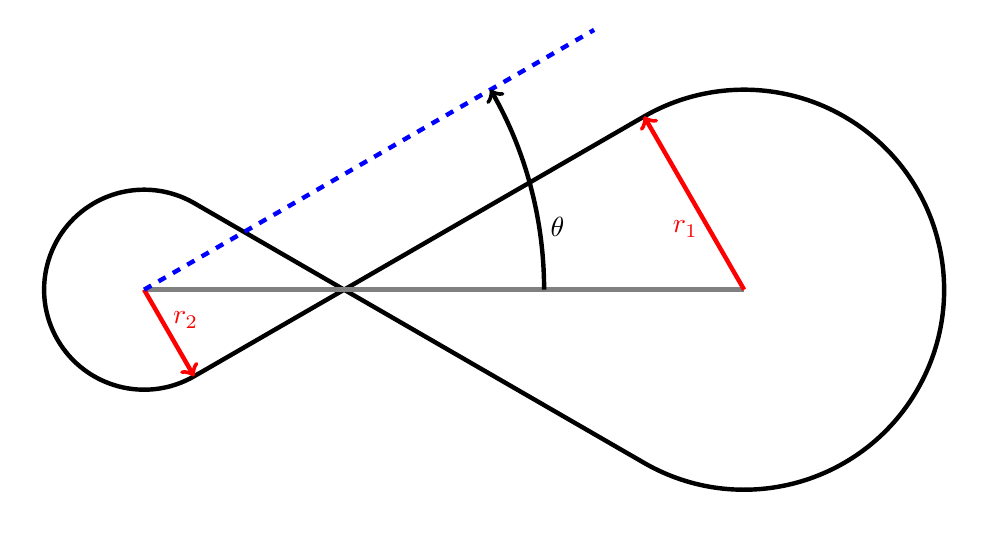
\begin{tikzpicture}[x=1.0in,y=1.0in]
		\draw[black, ultra thick] (.25, .433) -- (2.5, -.866) arc (-120:120:1) -- (.25, -.433) arc (300:60:0.5) -- cycle;
		\draw[gray, ultra thick]   (0,0) -- (3, 0);
		\draw[red, ultra thick, ->]   (3,0) -- (2.5, .866) node[pos=0.35, left]{$r_1$};
		\draw[red, ultra thick, ->]   (0,0) -- (0.25, -.433) node[pos=0.35, right]{$r_2$};
		\draw[blue, ultra thick, dashed]   (0,0) -- (2.25, 1.299);
		\draw[black, ultra thick, ->] (2,0) arc(0:30:2) node[pos=0.3, right]{$\theta$};
		
	\end{tikzpicture}
	\caption{Belt Dimensions, Labeled}
	\end{figure}

	The belt angle now is

	\begin{align}
		sin(theta) = \frac{r_2 + r_1}{C} 
	\end{align}

	\begin{align}
		L = 2 \frac{C}{cos(\theta)} + r_1 (\pi + 2 \theta) + r_2 (\pi + 2 \theta)
	\end{align}

	Resulting in:

	\begin{align}
		L = \frac{2 C}{\sqrt{1 - (\frac{d_2 + d_1}{2 C})^2}} + \frac{d_1 + d_2}{2} (\pi + 2 \theta)
	\end{align}

	\section*{Belt Strength Calculation}

	Belt strength is calculated from the tables in the \href{https://www.gates.com/content/dam/gates/home/resources/resource-library/catalogs/light-power-and-precision-manual.pdf}{\underline{Gates Light Power and Precision Manual}}.

	These tables list allowable pulley torque $T(\omega, N)$ as a function of RPM $\omega$ and pulley teeth $N$. Note that 6 teeth should be in engagement.
	2-D interpolation is used to determine values on the in-betweens.
	Tabulated values outside the bounds are extrapolated. Omitted values are presumed to be zero.
	The multiplier factors are used to determine strength of different width belts.
	
	
\end{document}